% Options for packages loaded elsewhere
\PassOptionsToPackage{unicode}{hyperref}
\PassOptionsToPackage{hyphens}{url}
%
\documentclass[
]{book}
\usepackage{amsmath,amssymb}
\usepackage{lmodern}
\usepackage{iftex}
\ifPDFTeX
  \usepackage[T1]{fontenc}
  \usepackage[utf8]{inputenc}
  \usepackage{textcomp} % provide euro and other symbols
\else % if luatex or xetex
  \usepackage{unicode-math}
  \defaultfontfeatures{Scale=MatchLowercase}
  \defaultfontfeatures[\rmfamily]{Ligatures=TeX,Scale=1}
\fi
% Use upquote if available, for straight quotes in verbatim environments
\IfFileExists{upquote.sty}{\usepackage{upquote}}{}
\IfFileExists{microtype.sty}{% use microtype if available
  \usepackage[]{microtype}
  \UseMicrotypeSet[protrusion]{basicmath} % disable protrusion for tt fonts
}{}
\makeatletter
\@ifundefined{KOMAClassName}{% if non-KOMA class
  \IfFileExists{parskip.sty}{%
    \usepackage{parskip}
  }{% else
    \setlength{\parindent}{0pt}
    \setlength{\parskip}{6pt plus 2pt minus 1pt}}
}{% if KOMA class
  \KOMAoptions{parskip=half}}
\makeatother
\usepackage{xcolor}
\IfFileExists{xurl.sty}{\usepackage{xurl}}{} % add URL line breaks if available
\IfFileExists{bookmark.sty}{\usepackage{bookmark}}{\usepackage{hyperref}}
\hypersetup{
  pdftitle={Вежби од Statistical Rethinking},
  pdfauthor={Novica Nakov},
  hidelinks,
  pdfcreator={LaTeX via pandoc}}
\urlstyle{same} % disable monospaced font for URLs
\usepackage{color}
\usepackage{fancyvrb}
\newcommand{\VerbBar}{|}
\newcommand{\VERB}{\Verb[commandchars=\\\{\}]}
\DefineVerbatimEnvironment{Highlighting}{Verbatim}{commandchars=\\\{\}}
% Add ',fontsize=\small' for more characters per line
\usepackage{framed}
\definecolor{shadecolor}{RGB}{248,248,248}
\newenvironment{Shaded}{\begin{snugshade}}{\end{snugshade}}
\newcommand{\AlertTok}[1]{\textcolor[rgb]{0.94,0.16,0.16}{#1}}
\newcommand{\AnnotationTok}[1]{\textcolor[rgb]{0.56,0.35,0.01}{\textbf{\textit{#1}}}}
\newcommand{\AttributeTok}[1]{\textcolor[rgb]{0.77,0.63,0.00}{#1}}
\newcommand{\BaseNTok}[1]{\textcolor[rgb]{0.00,0.00,0.81}{#1}}
\newcommand{\BuiltInTok}[1]{#1}
\newcommand{\CharTok}[1]{\textcolor[rgb]{0.31,0.60,0.02}{#1}}
\newcommand{\CommentTok}[1]{\textcolor[rgb]{0.56,0.35,0.01}{\textit{#1}}}
\newcommand{\CommentVarTok}[1]{\textcolor[rgb]{0.56,0.35,0.01}{\textbf{\textit{#1}}}}
\newcommand{\ConstantTok}[1]{\textcolor[rgb]{0.00,0.00,0.00}{#1}}
\newcommand{\ControlFlowTok}[1]{\textcolor[rgb]{0.13,0.29,0.53}{\textbf{#1}}}
\newcommand{\DataTypeTok}[1]{\textcolor[rgb]{0.13,0.29,0.53}{#1}}
\newcommand{\DecValTok}[1]{\textcolor[rgb]{0.00,0.00,0.81}{#1}}
\newcommand{\DocumentationTok}[1]{\textcolor[rgb]{0.56,0.35,0.01}{\textbf{\textit{#1}}}}
\newcommand{\ErrorTok}[1]{\textcolor[rgb]{0.64,0.00,0.00}{\textbf{#1}}}
\newcommand{\ExtensionTok}[1]{#1}
\newcommand{\FloatTok}[1]{\textcolor[rgb]{0.00,0.00,0.81}{#1}}
\newcommand{\FunctionTok}[1]{\textcolor[rgb]{0.00,0.00,0.00}{#1}}
\newcommand{\ImportTok}[1]{#1}
\newcommand{\InformationTok}[1]{\textcolor[rgb]{0.56,0.35,0.01}{\textbf{\textit{#1}}}}
\newcommand{\KeywordTok}[1]{\textcolor[rgb]{0.13,0.29,0.53}{\textbf{#1}}}
\newcommand{\NormalTok}[1]{#1}
\newcommand{\OperatorTok}[1]{\textcolor[rgb]{0.81,0.36,0.00}{\textbf{#1}}}
\newcommand{\OtherTok}[1]{\textcolor[rgb]{0.56,0.35,0.01}{#1}}
\newcommand{\PreprocessorTok}[1]{\textcolor[rgb]{0.56,0.35,0.01}{\textit{#1}}}
\newcommand{\RegionMarkerTok}[1]{#1}
\newcommand{\SpecialCharTok}[1]{\textcolor[rgb]{0.00,0.00,0.00}{#1}}
\newcommand{\SpecialStringTok}[1]{\textcolor[rgb]{0.31,0.60,0.02}{#1}}
\newcommand{\StringTok}[1]{\textcolor[rgb]{0.31,0.60,0.02}{#1}}
\newcommand{\VariableTok}[1]{\textcolor[rgb]{0.00,0.00,0.00}{#1}}
\newcommand{\VerbatimStringTok}[1]{\textcolor[rgb]{0.31,0.60,0.02}{#1}}
\newcommand{\WarningTok}[1]{\textcolor[rgb]{0.56,0.35,0.01}{\textbf{\textit{#1}}}}
\usepackage{longtable,booktabs,array}
\usepackage{calc} % for calculating minipage widths
% Correct order of tables after \paragraph or \subparagraph
\usepackage{etoolbox}
\makeatletter
\patchcmd\longtable{\par}{\if@noskipsec\mbox{}\fi\par}{}{}
\makeatother
% Allow footnotes in longtable head/foot
\IfFileExists{footnotehyper.sty}{\usepackage{footnotehyper}}{\usepackage{footnote}}
\makesavenoteenv{longtable}
\usepackage{graphicx}
\makeatletter
\def\maxwidth{\ifdim\Gin@nat@width>\linewidth\linewidth\else\Gin@nat@width\fi}
\def\maxheight{\ifdim\Gin@nat@height>\textheight\textheight\else\Gin@nat@height\fi}
\makeatother
% Scale images if necessary, so that they will not overflow the page
% margins by default, and it is still possible to overwrite the defaults
% using explicit options in \includegraphics[width, height, ...]{}
\setkeys{Gin}{width=\maxwidth,height=\maxheight,keepaspectratio}
% Set default figure placement to htbp
\makeatletter
\def\fps@figure{htbp}
\makeatother
\setlength{\emergencystretch}{3em} % prevent overfull lines
\providecommand{\tightlist}{%
  \setlength{\itemsep}{0pt}\setlength{\parskip}{0pt}}
\setcounter{secnumdepth}{5}
\usepackage{booktabs}
\ifLuaTeX
  \usepackage{selnolig}  % disable illegal ligatures
\fi
\usepackage[]{natbib}
\bibliographystyle{plainnat}

\title{Вежби од Statistical Rethinking}
\author{Novica Nakov}
\date{2022-01-21}

\begin{document}
\maketitle

{
\setcounter{tocdepth}{1}
\tableofcontents
}
\hypertarget{ux437ux430-ux43eux432ux43eux458-bookdown-ux43fux440ux43eux435ux43aux442}{%
\chapter{За овој bookdown проект}\label{ux437ux430-ux43eux432ux43eux458-bookdown-ux43fux440ux43eux435ux43aux442}}

Statistical Rethinking e популарна книга за учење моделирање на податоци. Предавањата се \href{https://github.com/rmcelreath/stat_rethinking_2022}{јавно достапни} и одлични. Ова се вежбите и моите решенија од книгата (која што може да се најде на интернет во PDF).

Текстот ќе биде измешан на македонски и англиски. Вежбите се ископирани од книгата и на англиски. Некои мои дообјаснувања и размислувања можеби ќе бидат на англиски, а можеби на македонски.

Моето читање на книгата и следење на предавањата коинцидира со \href{https://r4ds.github.io/bookclub-statrethink/}{клубот на R4DS}. Содржините таму се целосно на англиски.

\hypertarget{small-worlds-and-large-worlds}{%
\chapter{Small Worlds and Large Worlds}\label{small-worlds-and-large-worlds}}

Exercises from Chapter 2 of the book.

\begin{Shaded}
\begin{Highlighting}[]
\FunctionTok{library}\NormalTok{(tidyverse)}
\FunctionTok{library}\NormalTok{(patchwork)}
\end{Highlighting}
\end{Shaded}

\emph{2M1. Recall the globe tossing model from the chapter. Compute and plot the grid approximate posterior distribution for each of the following sets of observations. In each case, assume a uniform prior for p.}
\emph{1. W, W, W}
\emph{2. W, W, W, L}
\emph{3. L, W, W, L, W, W, W}

There are three datasets for this problem. Let's store them in a list for ease of work below.

\begin{Shaded}
\begin{Highlighting}[]
\NormalTok{data\_1 }\OtherTok{\textless{}{-}} \FunctionTok{c}\NormalTok{(}\StringTok{"W"}\NormalTok{, }\StringTok{"W"}\NormalTok{, }\StringTok{"W"}\NormalTok{)}
\NormalTok{data\_2 }\OtherTok{\textless{}{-}} \FunctionTok{c}\NormalTok{(}\StringTok{"W"}\NormalTok{, }\StringTok{"W"}\NormalTok{, }\StringTok{"W"}\NormalTok{, }\StringTok{"L"}\NormalTok{)}
\NormalTok{data\_3 }\OtherTok{\textless{}{-}} \FunctionTok{c}\NormalTok{(}\StringTok{"L"}\NormalTok{, }\StringTok{"W"}\NormalTok{, }\StringTok{"W"}\NormalTok{, }\StringTok{"L"}\NormalTok{, }\StringTok{"W"}\NormalTok{, }\StringTok{"W"}\NormalTok{, }\StringTok{"W"}\NormalTok{)}
\NormalTok{data\_lst }\OtherTok{\textless{}{-}} \FunctionTok{list}\NormalTok{(data\_1, data\_2, data\_3)}
\FunctionTok{names}\NormalTok{(data\_lst) }\OtherTok{\textless{}{-}} \FunctionTok{c}\NormalTok{(}\StringTok{"data\_1"}\NormalTok{, }\StringTok{"data\_2"}\NormalTok{, }\StringTok{"data\_3"}\NormalTok{)}
\end{Highlighting}
\end{Shaded}

\begin{Shaded}
\begin{Highlighting}[]
\CommentTok{\# define grid same for all}
\NormalTok{p\_grid }\OtherTok{\textless{}{-}} \FunctionTok{seq}\NormalTok{(}\AttributeTok{from =} \DecValTok{0}\NormalTok{, }\AttributeTok{to =} \DecValTok{1}\NormalTok{, }\AttributeTok{length.out =} \DecValTok{1000}\NormalTok{)}

\CommentTok{\# define prior same for all}
\NormalTok{prob\_p }\OtherTok{\textless{}{-}} \FunctionTok{rep}\NormalTok{(}\DecValTok{1}\NormalTok{, }\DecValTok{1000}\NormalTok{)}

\CommentTok{\#compute posterior }

\NormalTok{posterior }\OtherTok{\textless{}{-}} \ControlFlowTok{function}\NormalTok{(data, p\_grid, prob\_p, }\AttributeTok{plot =} \ConstantTok{TRUE}\NormalTok{) \{}
  
\CommentTok{\# compute likelihood at each value in grid}
\NormalTok{prob\_data }\OtherTok{\textless{}{-}} \FunctionTok{dbinom}\NormalTok{( }
  \FunctionTok{sum}\NormalTok{(data }\SpecialCharTok{==} \StringTok{"W"}\NormalTok{), }
  \AttributeTok{size=}\FunctionTok{length}\NormalTok{(data) , }
  \AttributeTok{prob=}\NormalTok{p\_grid )}
\CommentTok{\# compute product of likelihood and prior}
\NormalTok{posterior }\OtherTok{\textless{}{-}}\NormalTok{ prob\_data }\SpecialCharTok{*}\NormalTok{ prob\_p}
\CommentTok{\# standardize the posterior, so it sums to 1}
\NormalTok{posterior }\OtherTok{\textless{}{-}}\NormalTok{ posterior }\SpecialCharTok{/} \FunctionTok{sum}\NormalTok{(posterior)}

\NormalTok{data\_for\_plot }\OtherTok{\textless{}{-}} \FunctionTok{data.frame}\NormalTok{(}\AttributeTok{param =}\NormalTok{ p\_grid, }\AttributeTok{posterior =}\NormalTok{ posterior)}

\ControlFlowTok{if}\NormalTok{ (plot) \{}
\NormalTok{ p }\OtherTok{\textless{}{-}}  \FunctionTok{ggplot}\NormalTok{(data\_for\_plot) }\SpecialCharTok{+} 
   \FunctionTok{aes}\NormalTok{(}\AttributeTok{x =}\NormalTok{ param, }\AttributeTok{y =}\NormalTok{ posterior ) }\SpecialCharTok{+} 
   \FunctionTok{geom\_line}\NormalTok{() }\SpecialCharTok{+}
   \FunctionTok{labs}\NormalTok{(}\AttributeTok{x =} \StringTok{"Proportion of Water"}\NormalTok{, }\AttributeTok{y =} \StringTok{"Posterior Probability"}\NormalTok{) }\SpecialCharTok{+} 
   \FunctionTok{theme\_minimal}\NormalTok{()}
\NormalTok{ p}
\NormalTok{\} }\ControlFlowTok{else}\NormalTok{ \{}
\NormalTok{  posterior}
\NormalTok{\}}

\NormalTok{\}}


\NormalTok{plots }\OtherTok{\textless{}{-}} \FunctionTok{lapply}\NormalTok{(data\_lst, posterior, p\_grid, prob\_p)}

\NormalTok{plots[[}\DecValTok{1}\NormalTok{]]}\SpecialCharTok{+}\NormalTok{ plots[[}\DecValTok{2}\NormalTok{]]}\SpecialCharTok{+}\NormalTok{ plots[[}\DecValTok{3}\NormalTok{]]}
\end{Highlighting}
\end{Shaded}

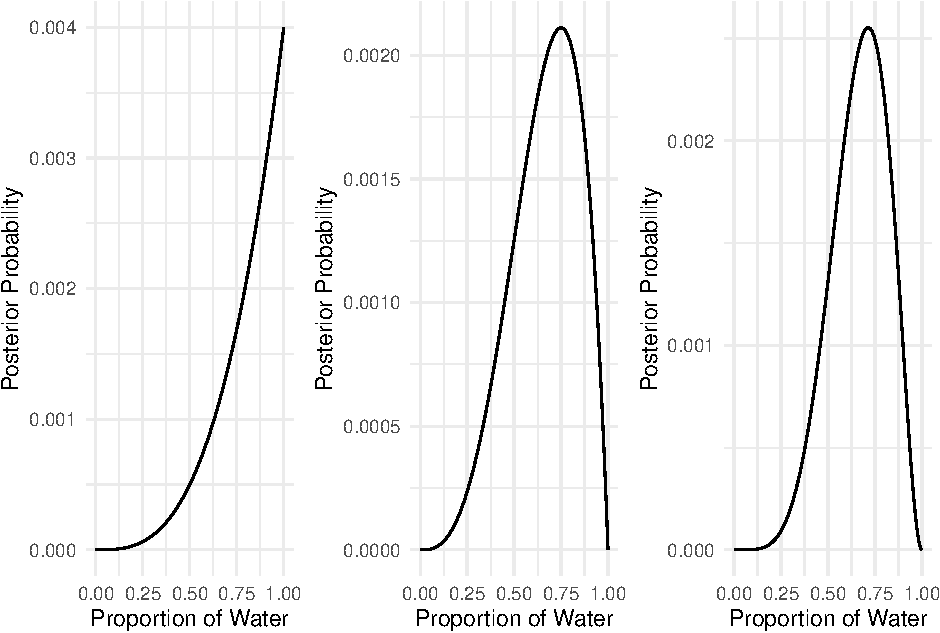
\includegraphics{_main_files/figure-latex/solve_2M1-1.pdf}

\emph{2M2. Now assume a prior for p that is equal to zero when p \textless{} 0.5 and is a positive constant when p ≥ 0.5. Again compute and plot the grid approximate posterior distribution for each of the sets of observations in the problem just above.}

Exercise 2M2 is basically the same as 2M1. The only difference is the prior. Let's try it with a more of a tidyverse solution.

\begin{Shaded}
\begin{Highlighting}[]
\NormalTok{data\_for\_plots }\OtherTok{\textless{}{-}}
  \FunctionTok{tibble}\NormalTok{(}\AttributeTok{p\_grid =} \FunctionTok{seq}\NormalTok{(}\AttributeTok{from =} \DecValTok{0}\NormalTok{, }\AttributeTok{to =} \DecValTok{1}\NormalTok{, }\AttributeTok{length.out =} \DecValTok{1000}\NormalTok{)) }\SpecialCharTok{\%\textgreater{}\%}     
  \FunctionTok{mutate}\NormalTok{(}\AttributeTok{prior =} \FunctionTok{if\_else}\NormalTok{(p\_grid }\SpecialCharTok{\textless{}} \FloatTok{0.5}\NormalTok{, }\DecValTok{0}\NormalTok{, }\DecValTok{1}\NormalTok{)) }\SpecialCharTok{\%\textgreater{}\%} 
  \FunctionTok{mutate}\NormalTok{(}\AttributeTok{data\_1 =} \FunctionTok{dbinom}\NormalTok{(}\FunctionTok{sum}\NormalTok{(data\_1 }\SpecialCharTok{==} \StringTok{"W"}\NormalTok{), }\AttributeTok{size=}\FunctionTok{length}\NormalTok{(data\_1), }\AttributeTok{prob =}\NormalTok{ p\_grid)) }\SpecialCharTok{\%\textgreater{}\%}
  \FunctionTok{mutate}\NormalTok{(}\AttributeTok{data\_2 =} \FunctionTok{dbinom}\NormalTok{(}\FunctionTok{sum}\NormalTok{(data\_2 }\SpecialCharTok{==} \StringTok{"W"}\NormalTok{), }\AttributeTok{size=}\FunctionTok{length}\NormalTok{(data\_2), }\AttributeTok{prob =}\NormalTok{ p\_grid)) }\SpecialCharTok{\%\textgreater{}\%}
  \FunctionTok{mutate}\NormalTok{(}\AttributeTok{data\_3 =} \FunctionTok{dbinom}\NormalTok{(}\FunctionTok{sum}\NormalTok{(data\_3 }\SpecialCharTok{==} \StringTok{"W"}\NormalTok{), }\AttributeTok{size=}\FunctionTok{length}\NormalTok{(data\_3), }\AttributeTok{prob =}\NormalTok{ p\_grid)) }\SpecialCharTok{\%\textgreater{}\%}
  \FunctionTok{pivot\_longer}\NormalTok{(}
    \AttributeTok{cols =} \FunctionTok{starts\_with}\NormalTok{(}\StringTok{"data"}\NormalTok{),}
    \AttributeTok{names\_to =} \StringTok{"data"}\NormalTok{,}
    \AttributeTok{values\_to =} \StringTok{"observations"}
\NormalTok{  ) }\SpecialCharTok{\%\textgreater{}\%} 
  \FunctionTok{mutate}\NormalTok{(}\AttributeTok{unstd\_posterior =}\NormalTok{ observations }\SpecialCharTok{*}\NormalTok{ prior) }\SpecialCharTok{\%\textgreater{}\%}           
  \FunctionTok{mutate}\NormalTok{(}\AttributeTok{posterior =}\NormalTok{ unstd\_posterior }\SpecialCharTok{/} \FunctionTok{sum}\NormalTok{(unstd\_posterior))}



\FunctionTok{ggplot}\NormalTok{(data\_for\_plots) }\SpecialCharTok{+}
  \FunctionTok{aes}\NormalTok{(}\AttributeTok{x =}\NormalTok{ p\_grid, }\AttributeTok{y =}\NormalTok{ posterior) }\SpecialCharTok{+}
  \FunctionTok{geom\_line}\NormalTok{() }\SpecialCharTok{+}
  \FunctionTok{labs}\NormalTok{(}\AttributeTok{x =} \StringTok{"Proportion of Water"}\NormalTok{, }\AttributeTok{y =} \StringTok{"Posterior Probability"}\NormalTok{) }\SpecialCharTok{+}  
  \FunctionTok{theme\_minimal}\NormalTok{() }\SpecialCharTok{+}
  \FunctionTok{facet\_wrap}\NormalTok{(}\FunctionTok{vars}\NormalTok{(data), }\AttributeTok{nrow =} \DecValTok{1}\NormalTok{)}
\end{Highlighting}
\end{Shaded}

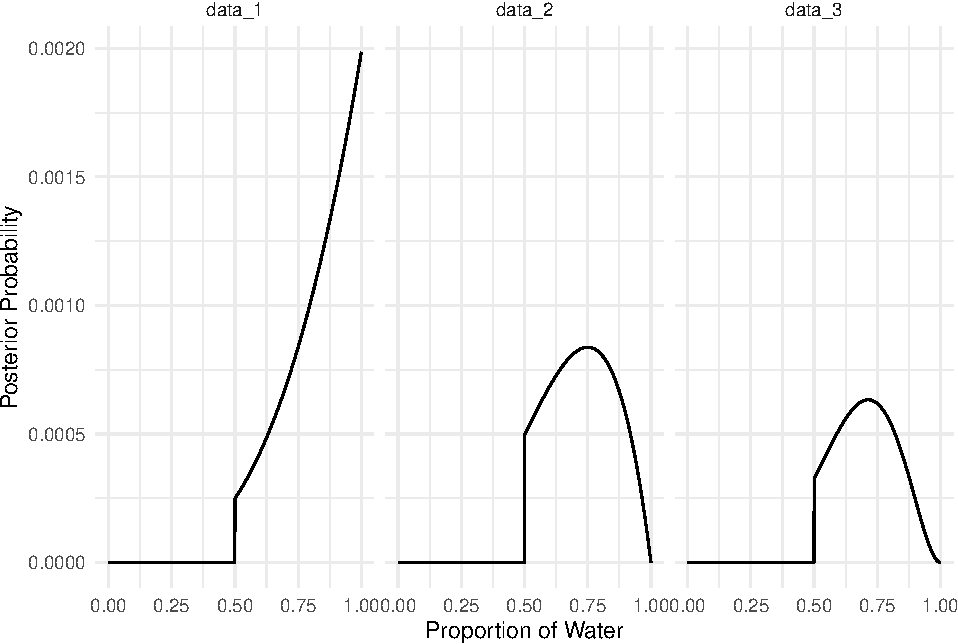
\includegraphics{_main_files/figure-latex/solve_2M2-1.pdf}

\emph{2M3. Suppose there are two globes, one for Earth and one for Mars. The Earth globe is 70\% covered in water. The Mars globe is 100\% land. Further suppose that one of these globes---you don't know which---was tossed in the air and produced a ``land'' observation. Assume that each globe was equally likely to be tossed. Show that the posterior probability that the globe was the Earth, conditional on seeing ``land'' (Pr(Earth\textbar land)), is 0.23.}1

\(Pr(Earth|land) = 0.23\)

\(Pr(Earth) = Pr(Mars) = 0.5\)

\(Pr(land|Earth) = 1 - 0.7 = 0.3\)

\(Pr(land|Mars) = 1\)

\textbf{Bayes theorem:}

\(Pr(Earth|land) = Pr(land|Earth) * Pr(Earth) / Pr(land|Earth) * Pr(Earth) + Pr(land|Mars) * Pr(Mars)\)

\begin{Shaded}
\begin{Highlighting}[]
\NormalTok{pr\_earth\_given\_land }\OtherTok{\textless{}{-}} \FloatTok{0.3} \SpecialCharTok{*} \FloatTok{0.5} \SpecialCharTok{/}\NormalTok{ (}\FloatTok{0.3} \SpecialCharTok{*} \FloatTok{0.5} \SpecialCharTok{+} \DecValTok{1} \SpecialCharTok{*} \FloatTok{0.5}\NormalTok{)}

\NormalTok{pr\_earth\_given\_land}
\end{Highlighting}
\end{Shaded}

\begin{verbatim}
## [1] 0.2307692
\end{verbatim}

\emph{2M4. Suppose you have a deck with only three cards. Each card has two sides, and each side is either black or white. One card has two black sides. The second card has one black and one white side. The third card has two white sides. Now suppose all three cards are placed in a bag and shuffled. Someone reaches into the bag and pulls out a card and places it flat on a table. A black side is shown facing up, but you don't know the color of the side facing down. Show that the probability that the other side is also black is 2/3. Use the counting method (Section 2 of the chapter) to approach this problem. This means counting up the ways that each card could produce the observed data (a black side facing up on the table).}

\begin{Shaded}
\begin{Highlighting}[]
\NormalTok{bb\_ways }\OtherTok{\textless{}{-}} \DecValTok{2}
\NormalTok{wb\_ways }\OtherTok{\textless{}{-}} \DecValTok{1}
\NormalTok{ww\_ways }\OtherTok{\textless{}{-}} \DecValTok{0}
\NormalTok{data }\OtherTok{\textless{}{-}} \FunctionTok{c}\NormalTok{(bb\_ways, wb\_ways, ww\_ways)}
\NormalTok{prior }\OtherTok{\textless{}{-}} \FunctionTok{c}\NormalTok{(}\DecValTok{1}\NormalTok{, }\DecValTok{1}\NormalTok{, }\DecValTok{1}\NormalTok{)}
\NormalTok{posterior }\OtherTok{\textless{}{-}}\NormalTok{ prior }\SpecialCharTok{*}\NormalTok{ data}
\NormalTok{posterior }\OtherTok{\textless{}{-}}\NormalTok{ posterior }\SpecialCharTok{/} \FunctionTok{sum}\NormalTok{(posterior)}
\NormalTok{posterior[}\DecValTok{1}\NormalTok{] }\SpecialCharTok{==} \DecValTok{2} \SpecialCharTok{/} \DecValTok{3}
\end{Highlighting}
\end{Shaded}

\begin{verbatim}
## [1] TRUE
\end{verbatim}

\emph{2M5. Now suppose there are four cards: B/B, B/W, W/W, and another B/B. Again suppose a card is drawn from the bag and a black side appears face up. Again calculate the probability that the other side is black.}

\begin{Shaded}
\begin{Highlighting}[]
\NormalTok{bb\_ways }\OtherTok{\textless{}{-}} \DecValTok{2}
\NormalTok{wb\_ways }\OtherTok{\textless{}{-}} \DecValTok{1}
\NormalTok{ww\_ways }\OtherTok{\textless{}{-}} \DecValTok{0}
\NormalTok{data }\OtherTok{\textless{}{-}} \FunctionTok{c}\NormalTok{(bb\_ways, wb\_ways, ww\_ways)}
\NormalTok{prior }\OtherTok{\textless{}{-}} \FunctionTok{c}\NormalTok{(}\DecValTok{2}\NormalTok{, }\DecValTok{1}\NormalTok{, }\DecValTok{1}\NormalTok{)}
\NormalTok{posterior }\OtherTok{\textless{}{-}}\NormalTok{ prior }\SpecialCharTok{*}\NormalTok{ data}
\NormalTok{posterior }\OtherTok{\textless{}{-}}\NormalTok{ posterior }\SpecialCharTok{/} \FunctionTok{sum}\NormalTok{(posterior)}

\NormalTok{posterior[}\DecValTok{1}\NormalTok{]}
\end{Highlighting}
\end{Shaded}

\begin{verbatim}
## [1] 0.8
\end{verbatim}

\emph{2M6. Imagine that black ink is heavy, and so cards with black sides are heavier than cards with white sides. As a result, it's less likely that a card with black sides is pulled from the bag. So again assume there are three cards: B/B, B/W, and W/W. After experimenting a number of times, you conclude that for every way to pull the B/B card from the bag, there are 2 ways to pull the B/W card and 3 ways to pull the W/W card. Again suppose that a card is pulled and a black side appears face up. Show that the probability the other side is black is now 0.5. Use the counting method, as before.}

\begin{Shaded}
\begin{Highlighting}[]
\NormalTok{bb\_ways }\OtherTok{\textless{}{-}} \DecValTok{2}
\NormalTok{wb\_ways }\OtherTok{\textless{}{-}} \DecValTok{1}
\NormalTok{ww\_ways }\OtherTok{\textless{}{-}} \DecValTok{0}
\NormalTok{data }\OtherTok{\textless{}{-}} \FunctionTok{c}\NormalTok{(bb\_ways, wb\_ways, ww\_ways)}
\NormalTok{prior }\OtherTok{\textless{}{-}} \FunctionTok{c}\NormalTok{(}\DecValTok{1}\NormalTok{, }\DecValTok{2}\NormalTok{, }\DecValTok{3}\NormalTok{)}
\NormalTok{posterior }\OtherTok{\textless{}{-}}\NormalTok{ prior }\SpecialCharTok{*}\NormalTok{ data}
\NormalTok{posterior }\OtherTok{\textless{}{-}}\NormalTok{ posterior }\SpecialCharTok{/} \FunctionTok{sum}\NormalTok{(posterior)}

\NormalTok{posterior[}\DecValTok{1}\NormalTok{] }\SpecialCharTok{==} \FloatTok{0.5}
\end{Highlighting}
\end{Shaded}

\begin{verbatim}
## [1] TRUE
\end{verbatim}

\emph{2M7. Assume again the original card problem, with a single card showing a black side face up. Before looking at the other side, we draw another card from the bag and lay it face up on the table. The face that is shown on the new card is white. Show that the probability that the first card, the one showing a black side, has black on its other side is now 0.75. Use the counting method, if you can. Hint: Treat this like the sequence of globe tosses, counting all the ways to see each observation, for each possible first card.}

\begin{Shaded}
\begin{Highlighting}[]
\NormalTok{bb\_ways }\OtherTok{\textless{}{-}} \DecValTok{2}\SpecialCharTok{*}\DecValTok{3}
\NormalTok{wb\_ways }\OtherTok{\textless{}{-}} \DecValTok{1}\SpecialCharTok{*}\DecValTok{2}
\NormalTok{ww\_ways }\OtherTok{\textless{}{-}} \DecValTok{0}\SpecialCharTok{*}\DecValTok{1}
\NormalTok{data }\OtherTok{\textless{}{-}} \FunctionTok{c}\NormalTok{(bb\_ways, wb\_ways, ww\_ways)}
\NormalTok{prior }\OtherTok{\textless{}{-}} \FunctionTok{c}\NormalTok{(}\DecValTok{1}\NormalTok{, }\DecValTok{1}\NormalTok{, }\DecValTok{1}\NormalTok{)}
\NormalTok{posterior }\OtherTok{\textless{}{-}}\NormalTok{ prior }\SpecialCharTok{*}\NormalTok{ data}
\NormalTok{posterior }\OtherTok{\textless{}{-}}\NormalTok{ posterior }\SpecialCharTok{/} \FunctionTok{sum}\NormalTok{(posterior)}

\NormalTok{posterior[}\DecValTok{1}\NormalTok{] }\SpecialCharTok{==} \FloatTok{0.75}
\end{Highlighting}
\end{Shaded}

\begin{verbatim}
## [1] TRUE
\end{verbatim}

\emph{2H1. Suppose there are two species of panda bear. Both are equally common in the wild and live in the same places. They look exactly alike and eat the same food, and there is yet no genetic assay capable of telling them apart. They differ however in their family sizes. Species A gives birth to twins 10\% of the time, otherwise birthing a single infant. Species B births twins 20\% of the time, otherwise birthing singleton infants. Assume these numbers are known with certainty, from many years of field research.}

\emph{Now suppose you are managing a captive panda breeding program. You have a new female panda of unknown species, and she has just given birth to twins. What is the probability that her next birth will also be twins?}

Прашањето е, која е веројатноста второто раѓање да е близнаци, кога првото било близнаци, или:

\(Pr(twins2|twins1) = ?\)

Треба да пресметаме:

\(Pr(twins2|twins1) = Pr(twins1, twins2) / Pr(twins)\)

Знаме дека:

\(Pr(twins|A) = 0.1\)

\(Pr(twins|B) = 0.2\)

\(Pr(A) = Pr(B) = 0.5\)

Треба да пресметаме и:

\(Pr(twins) = Pr(twins|A)*Pr(A) + Pr(twins|B)*Pr(B)\)

\$Pr(twins1, twins2) = Pr(twins\textbar A) * Pr(twins\textbar A) * Pr(A) + Pr(twins\textbar B) * Pr(twins\textbar B) * Pr(B) \$

\begin{Shaded}
\begin{Highlighting}[]
\NormalTok{pr\_twins }\OtherTok{\textless{}{-}} \FloatTok{0.1} \SpecialCharTok{*} \FloatTok{0.5} \SpecialCharTok{+} \FloatTok{0.2} \SpecialCharTok{*} \FloatTok{0.5}

\NormalTok{pr\_twins1\_and\_twins2 }\OtherTok{\textless{}{-}} \FloatTok{0.1} \SpecialCharTok{*} \FloatTok{0.1} \SpecialCharTok{*} \FloatTok{0.5} \SpecialCharTok{+} \FloatTok{0.2} \SpecialCharTok{*} \FloatTok{0.2} \SpecialCharTok{*} \FloatTok{0.5} 

\NormalTok{pr\_twins\_2\_given\_twins1 }\OtherTok{\textless{}{-}}\NormalTok{ pr\_twins1\_and\_twins2 }\SpecialCharTok{/}\NormalTok{ pr\_twins}

\NormalTok{pr\_twins\_2\_given\_twins1}
\end{Highlighting}
\end{Shaded}

\begin{verbatim}
## [1] 0.1666667
\end{verbatim}

\emph{2H2. Recall all the facts from the problem above. Now compute the probability that the panda we have is from species A, assuming we have observed only the first birth and that it was twins.}

Ова прашање е:

\(Pr(A|twins1) = ?\)

Баезова теорема:

\(Pr(A|twins1) = Pr(twins1|A) * Pr(A) / Pr(twins)\)

Ова може лесно да го пресметаме како:

\begin{Shaded}
\begin{Highlighting}[]
\NormalTok{pr\_twins\_given\_a }\OtherTok{=} \FloatTok{0.1} \SpecialCharTok{*} \FloatTok{0.5} \SpecialCharTok{/}\NormalTok{ pr\_twins}

\NormalTok{pr\_twins\_given\_a}
\end{Highlighting}
\end{Shaded}

\begin{verbatim}
## [1] 0.3333333
\end{verbatim}

Слично, може да креираме пресметка со која одеднаш ќе ги добиеме двете веројатности, т.е.:

\(Pr(A|twins1)\) и \(Pr(B|twins1)\).

\begin{Shaded}
\begin{Highlighting}[]
\NormalTok{p\_twins\_A }\OtherTok{\textless{}{-}} \FloatTok{0.1}
\NormalTok{p\_twins\_B }\OtherTok{\textless{}{-}} \FloatTok{0.2}
\NormalTok{data\_twins }\OtherTok{\textless{}{-}} \FunctionTok{c}\NormalTok{(p\_twins\_A, p\_twins\_B)}
\NormalTok{prior }\OtherTok{\textless{}{-}} \FunctionTok{c}\NormalTok{(}\DecValTok{1}\NormalTok{, }\DecValTok{1}\NormalTok{)}
\NormalTok{posterior }\OtherTok{\textless{}{-}}\NormalTok{ prior }\SpecialCharTok{*}\NormalTok{ data\_twins}
\NormalTok{posterior\_2H2 }\OtherTok{\textless{}{-}}\NormalTok{ posterior }\SpecialCharTok{/} \FunctionTok{sum}\NormalTok{(posterior)}
\FunctionTok{names}\NormalTok{(posterior\_2H2) }\OtherTok{=} \FunctionTok{c}\NormalTok{(}\StringTok{"pr\_A\_twins"}\NormalTok{, }\StringTok{"pr\_B\_twins"}\NormalTok{)}
\NormalTok{posterior\_2H2}
\end{Highlighting}
\end{Shaded}

\begin{verbatim}
## pr_A_twins pr_B_twins 
##  0.3333333  0.6666667
\end{verbatim}

\emph{2H3. Continuing on from the previous problem, suppose the same panda mother has a second birth and that it is not twins, but a singleton infant. Compute the posterior probability that this panda is species A.}

Сега прашањето е за веројатноста пандата да е вид А ако родила прво близнаци, па потоа едно мече:

\(Pr(A|single) = ?\)

Овде може да се искористи \emph{bayеsian updating} бидејќи веќе имаме веројатност за А при раѓање близанци од претходната вежба, што ќе биде \emph{prior} т.е.:

\(Pr(A|twins) = 0.3\)

Новородената панда всушност ја третираме како нови податоци во пресметката

\begin{Shaded}
\begin{Highlighting}[]
\NormalTok{data\_single }\OtherTok{\textless{}{-}} \FunctionTok{c}\NormalTok{(}\DecValTok{1} \SpecialCharTok{{-}}\NormalTok{ p\_twins\_A, }\DecValTok{1} \SpecialCharTok{{-}}\NormalTok{ p\_twins\_B)}
\NormalTok{prior\_2H3 }\OtherTok{\textless{}{-}}\NormalTok{ posterior\_2H2}
\NormalTok{posterior }\OtherTok{\textless{}{-}}\NormalTok{ prior\_2H3 }\SpecialCharTok{*}\NormalTok{ data\_single}
\NormalTok{posterior\_2H3 }\OtherTok{\textless{}{-}}\NormalTok{ posterior }\SpecialCharTok{/} \FunctionTok{sum}\NormalTok{(posterior)}
\FunctionTok{names}\NormalTok{(posterior\_2H3) }\OtherTok{=} \FunctionTok{c}\NormalTok{(}\StringTok{"pr\_A\_single"}\NormalTok{, }\StringTok{"pr\_B\_single"}\NormalTok{)}
\NormalTok{posterior\_2H3}
\end{Highlighting}
\end{Shaded}

\begin{verbatim}
## pr_A_single pr_B_single 
##        0.36        0.64
\end{verbatim}

\emph{2H4. A common boast of Bayesian statisticians is that Bayesian inference makes it easy to use all of the data, even if the data are of different types.}

\emph{So suppose now that a veterinarian comes along who has a new genetic test that she claims can identify the species of our mother panda. But the test, like all tests, is imperfect. This is the information you have about the test:}

**The probability it correctly identifies a species A panda is 0.8.*
**The probability it correctly identifies a species B panda is 0.65.*

\emph{The vet administers the test to your panda and tells you that the test is positive for species A. First ignore your previous information from the births and compute the posterior probability that your panda is species A. Then redo your calculation, now using the birth data as well.}

Првото прашање е:

\(Pr(A|testA) = ?\)

Знаеме дека:

\(Pr(testA|A) = 0.8\)
\(Pr(testA|B) = 1 - 0.65 = 0.35\) тестот точно предвидува вид B 0.65 од случаите, значи, 0.35 се А.

\begin{Shaded}
\begin{Highlighting}[]
\NormalTok{test\_correct\_A }\OtherTok{\textless{}{-}} \FloatTok{0.8}
\NormalTok{test\_correct\_B }\OtherTok{\textless{}{-}} \FloatTok{0.35}
\NormalTok{data }\OtherTok{\textless{}{-}} \FunctionTok{c}\NormalTok{(test\_correct\_A, test\_correct\_B)}
\NormalTok{prior }\OtherTok{\textless{}{-}} \FunctionTok{c}\NormalTok{(}\DecValTok{1}\NormalTok{, }\DecValTok{1}\NormalTok{)}
\NormalTok{posterior }\OtherTok{\textless{}{-}}\NormalTok{ prior }\SpecialCharTok{*}\NormalTok{ data}
\NormalTok{posterior\_2H4 }\OtherTok{\textless{}{-}}\NormalTok{ posterior }\SpecialCharTok{/} \FunctionTok{sum}\NormalTok{(posterior)}
\FunctionTok{names}\NormalTok{(posterior\_2H4) }\OtherTok{=} \FunctionTok{c}\NormalTok{(}\StringTok{"panda\_is\_A"}\NormalTok{, }\StringTok{"panda\_is\_B"}\NormalTok{)}
\NormalTok{posterior\_2H4}
\end{Highlighting}
\end{Shaded}

\begin{verbatim}
## panda_is_A panda_is_B 
##  0.6956522  0.3043478
\end{verbatim}

Тука, слично како претходно, како \emph{prior} го сметаме резултатот т.е. \emph{posterior} од пресметката со раѓања.

\begin{Shaded}
\begin{Highlighting}[]
\NormalTok{prior }\OtherTok{\textless{}{-}}\NormalTok{ posterior\_2H3}
\NormalTok{posterior }\OtherTok{\textless{}{-}}\NormalTok{ prior }\SpecialCharTok{*}\NormalTok{ data}
\NormalTok{posterior\_2H4\_2 }\OtherTok{\textless{}{-}}\NormalTok{ posterior }\SpecialCharTok{/} \FunctionTok{sum}\NormalTok{(posterior)}
\FunctionTok{names}\NormalTok{(posterior\_2H4\_2) }\OtherTok{=} \FunctionTok{c}\NormalTok{(}\StringTok{"panda\_is\_A"}\NormalTok{, }\StringTok{"panda\_is\_B"}\NormalTok{)}
\NormalTok{posterior\_2H4\_2}
\end{Highlighting}
\end{Shaded}

\begin{verbatim}
## panda_is_A panda_is_B 
##     0.5625     0.4375
\end{verbatim}

На крај:

\(Pr(A|testA,twins,single) = 0.56\)

Веројатноста пандата да е вид А при точен тест за вид А, родени близнаци и потоа едно пандиче е околу 0.56.

\hypertarget{sampling-the-imaginary}{%
\chapter{Sampling the Imaginary}\label{sampling-the-imaginary}}

Exercises from Chapter 3 of the book.

\begin{Shaded}
\begin{Highlighting}[]
\FunctionTok{library}\NormalTok{(tidyverse)}
\FunctionTok{library}\NormalTok{(rethinking)}
\end{Highlighting}
\end{Shaded}

Лесните прашања го користат кодот од книгата и само правиме пресметки што се опишан во \emph{3.2. Sampling to summarize section} на книгата.

\begin{Shaded}
\begin{Highlighting}[]
\NormalTok{p\_grid }\OtherTok{\textless{}{-}} \FunctionTok{seq}\NormalTok{( }\AttributeTok{from=}\DecValTok{0}\NormalTok{ , }\AttributeTok{to=}\DecValTok{1}\NormalTok{ , }\AttributeTok{length.out=}\DecValTok{1000}\NormalTok{ )}
\NormalTok{prior }\OtherTok{\textless{}{-}} \FunctionTok{rep}\NormalTok{( }\DecValTok{1}\NormalTok{ , }\DecValTok{1000}\NormalTok{ )}
\NormalTok{likelihood }\OtherTok{\textless{}{-}} \FunctionTok{dbinom}\NormalTok{( }\DecValTok{6}\NormalTok{ , }\AttributeTok{size=}\DecValTok{9}\NormalTok{ , }\AttributeTok{prob=}\NormalTok{p\_grid )}
\NormalTok{posterior }\OtherTok{\textless{}{-}}\NormalTok{ likelihood }\SpecialCharTok{*}\NormalTok{ prior}
\NormalTok{posterior }\OtherTok{\textless{}{-}}\NormalTok{ posterior }\SpecialCharTok{/} \FunctionTok{sum}\NormalTok{(posterior)}
\FunctionTok{set.seed}\NormalTok{(}\DecValTok{100}\NormalTok{)}
\NormalTok{samples }\OtherTok{\textless{}{-}} \FunctionTok{sample}\NormalTok{( p\_grid , }\AttributeTok{prob=}\NormalTok{posterior , }\AttributeTok{size=}\FloatTok{1e4}\NormalTok{ , }\AttributeTok{replace=}\ConstantTok{TRUE}\NormalTok{ )}
\end{Highlighting}
\end{Shaded}

\emph{3E1. How much posterior probability lies below p = 0.2?}

\begin{Shaded}
\begin{Highlighting}[]
\FunctionTok{mean}\NormalTok{( samples }\SpecialCharTok{\textless{}} \FloatTok{0.2}\NormalTok{ )}
\end{Highlighting}
\end{Shaded}

\begin{verbatim}
## [1] 4e-04
\end{verbatim}

\emph{3E2. How much posterior probability lies above p = 0.8?}

\begin{Shaded}
\begin{Highlighting}[]
\FunctionTok{mean}\NormalTok{( samples }\SpecialCharTok{\textgreater{}} \FloatTok{0.8}\NormalTok{ )}
\end{Highlighting}
\end{Shaded}

\begin{verbatim}
## [1] 0.1116
\end{verbatim}

\emph{3E3. How much posterior probability lies between p = 0.2 and p = 0.8?}

\begin{Shaded}
\begin{Highlighting}[]
\FunctionTok{mean}\NormalTok{( samples }\SpecialCharTok{\textgreater{}} \FloatTok{0.2} \SpecialCharTok{\&}\NormalTok{ samples }\SpecialCharTok{\textless{}} \FloatTok{0.8}\NormalTok{ )}
\end{Highlighting}
\end{Shaded}

\begin{verbatim}
## [1] 0.888
\end{verbatim}

Аll three should be 1.

\begin{Shaded}
\begin{Highlighting}[]
\FunctionTok{sum}\NormalTok{(}\FunctionTok{mean}\NormalTok{( samples }\SpecialCharTok{\textless{}} \FloatTok{0.2}\NormalTok{ ), }\FunctionTok{mean}\NormalTok{( samples }\SpecialCharTok{\textgreater{}} \FloatTok{0.8}\NormalTok{ ), }\FunctionTok{mean}\NormalTok{( samples }\SpecialCharTok{\textgreater{}} \FloatTok{0.2} \SpecialCharTok{\&}\NormalTok{ samples }\SpecialCharTok{\textless{}} \FloatTok{0.8}\NormalTok{ ))}
\end{Highlighting}
\end{Shaded}

\begin{verbatim}
## [1] 1
\end{verbatim}

\emph{3E4. 20\% of the posterior probability lies below which value of p?}

\begin{Shaded}
\begin{Highlighting}[]
\FunctionTok{quantile}\NormalTok{(samples, }\FloatTok{0.2}\NormalTok{)}
\end{Highlighting}
\end{Shaded}

\begin{verbatim}
##       20% 
## 0.5185185
\end{verbatim}

\emph{3E5. 20\% of the posterior probability lies above which value of p?}

\begin{Shaded}
\begin{Highlighting}[]
\FunctionTok{quantile}\NormalTok{(samples, }\FloatTok{0.8}\NormalTok{)}
\end{Highlighting}
\end{Shaded}

\begin{verbatim}
##       80% 
## 0.7557558
\end{verbatim}

\emph{3E6. Which values of p contain the narrowest interval equal to 66\% of the posterior probability?}

\begin{Shaded}
\begin{Highlighting}[]
\FunctionTok{HPDI}\NormalTok{( samples , }\AttributeTok{prob=}\FloatTok{0.66}\NormalTok{ )}
\end{Highlighting}
\end{Shaded}

\begin{verbatim}
##     |0.66     0.66| 
## 0.5085085 0.7737738
\end{verbatim}

Trying the tidybayes functions. The results are the same.

\begin{Shaded}
\begin{Highlighting}[]
\NormalTok{tidybayes}\SpecialCharTok{::}\FunctionTok{mode\_hdi}\NormalTok{(samples, }\AttributeTok{.width =}\NormalTok{ .}\DecValTok{66}\NormalTok{)}
\end{Highlighting}
\end{Shaded}

\begin{verbatim}
##           y      ymin      ymax .width .point .interval
## 1 0.6477573 0.5085085 0.7737738   0.66   mode       hdi
\end{verbatim}

\begin{Shaded}
\begin{Highlighting}[]
\NormalTok{tidybayes}\SpecialCharTok{::}\FunctionTok{hdi}\NormalTok{(samples, }\AttributeTok{.width =}\NormalTok{ .}\DecValTok{66}\NormalTok{)}
\end{Highlighting}
\end{Shaded}

\begin{verbatim}
##           [,1]      [,2]
## [1,] 0.5085085 0.7737738
\end{verbatim}

\emph{3E7. Which values of p contain 66\% of the posterior probability, assuming equal posterior probability both below and above the interval?}

\begin{Shaded}
\begin{Highlighting}[]
\FunctionTok{PI}\NormalTok{(samples, }\AttributeTok{prob =} \FloatTok{0.66}\NormalTok{)}
\end{Highlighting}
\end{Shaded}

\begin{verbatim}
##       17%       83% 
## 0.5025025 0.7697698
\end{verbatim}

\emph{3M1. Suppose the globe tossing data had turned out to be 8 water in 15 tosses. Construct the posterior distribution, using grid approximation. Use the same flat prior as before.}

Ова е истиот проблем како лесните, единствено ги менуваме параметрите на \texttt{dbinom}.

\begin{Shaded}
\begin{Highlighting}[]
\NormalTok{p\_grid }\OtherTok{\textless{}{-}} \FunctionTok{seq}\NormalTok{(}\AttributeTok{from=}\DecValTok{0}\NormalTok{, }\AttributeTok{to=}\DecValTok{1}\NormalTok{, }\AttributeTok{length.out=}\DecValTok{1000}\NormalTok{)}
\NormalTok{prior }\OtherTok{\textless{}{-}} \FunctionTok{rep}\NormalTok{(}\DecValTok{1}\NormalTok{, }\DecValTok{1000}\NormalTok{)}
\NormalTok{likelihood }\OtherTok{\textless{}{-}} \FunctionTok{dbinom}\NormalTok{(}\DecValTok{8}\NormalTok{, }\AttributeTok{size=}\DecValTok{15}\NormalTok{, }\AttributeTok{prob=}\NormalTok{p\_grid)}
\NormalTok{posterior }\OtherTok{\textless{}{-}}\NormalTok{ likelihood }\SpecialCharTok{*}\NormalTok{ prior}
\NormalTok{posterior\_3m1 }\OtherTok{\textless{}{-}}\NormalTok{ posterior }\SpecialCharTok{/} \FunctionTok{sum}\NormalTok{(posterior)}

\FunctionTok{plot}\NormalTok{(posterior, }\AttributeTok{type =} \StringTok{"l"}\NormalTok{)}
\end{Highlighting}
\end{Shaded}

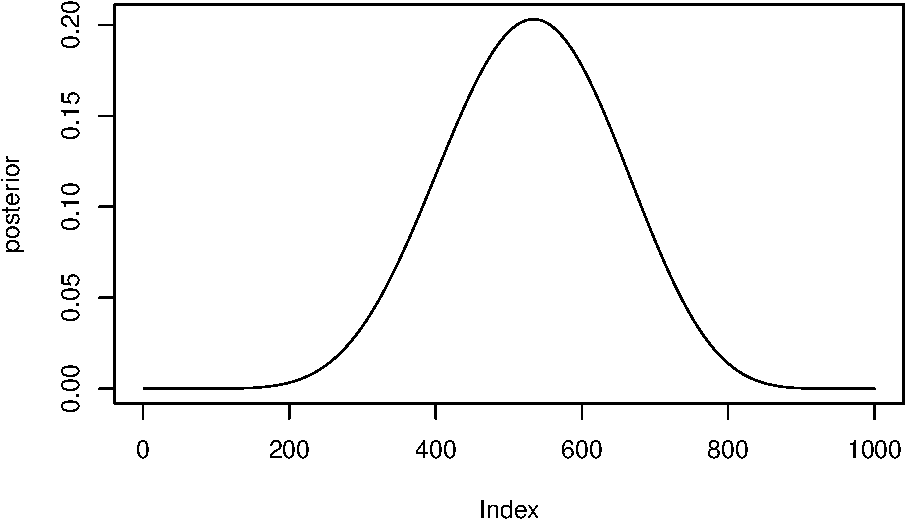
\includegraphics{_main_files/figure-latex/solve_3M1-1.pdf}

\emph{3M2. Draw 10,000 samples from the grid approximation from above. Then use the samples to calculate the 90\% HPDI for p.}

\begin{Shaded}
\begin{Highlighting}[]
\NormalTok{samples }\OtherTok{\textless{}{-}} \FunctionTok{sample}\NormalTok{( p\_grid , }\AttributeTok{prob=}\NormalTok{posterior\_3m1 , }\AttributeTok{size=}\FloatTok{1e4}\NormalTok{ , }\AttributeTok{replace=}\ConstantTok{TRUE}\NormalTok{ )}

\FunctionTok{HPDI}\NormalTok{( samples , }\AttributeTok{prob=}\FloatTok{0.9}\NormalTok{ )}
\end{Highlighting}
\end{Shaded}

\begin{verbatim}
##      |0.9      0.9| 
## 0.3293293 0.7167167
\end{verbatim}

\emph{3M3. Construct a posterior predictive check for this model and data. This means simulate the distribution of samples, averaging over the posterior uncertainty in p.}

Ова значи да симулираме податоци од моделот. Делот 3.3.2 од книгата.

\begin{Shaded}
\begin{Highlighting}[]
\FunctionTok{set.seed}\NormalTok{(}\DecValTok{123}\NormalTok{)}

\NormalTok{simulate\_w }\OtherTok{\textless{}{-}} \FunctionTok{rbinom}\NormalTok{( }\FloatTok{1e4}\NormalTok{ , }\AttributeTok{size=}\DecValTok{15}\NormalTok{ , }\AttributeTok{prob=}\NormalTok{samples )}

\FunctionTok{simplehist}\NormalTok{(simulate\_w)}
\end{Highlighting}
\end{Shaded}

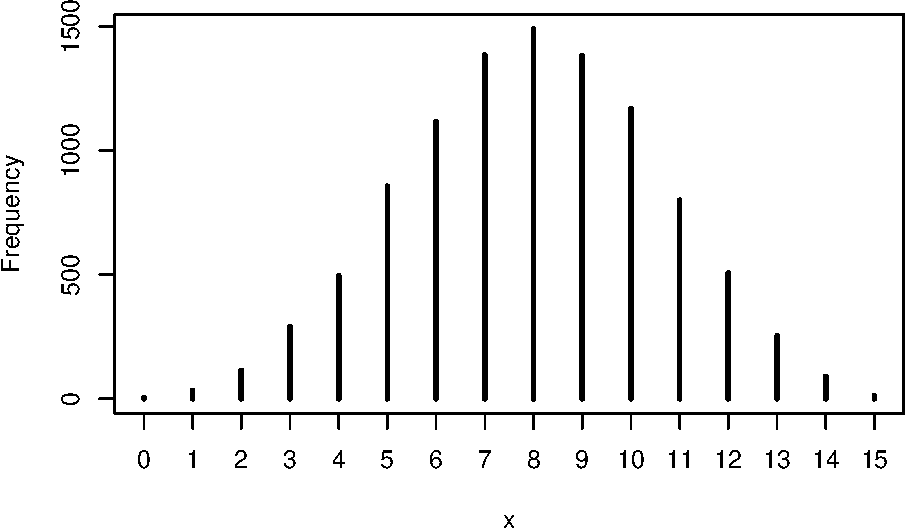
\includegraphics{_main_files/figure-latex/solve_3M3-1.pdf}

\emph{What is the probability of observing 8 water in 15 tosses?}

\begin{Shaded}
\begin{Highlighting}[]
\FunctionTok{mean}\NormalTok{(simulate\_w }\SpecialCharTok{==} \DecValTok{8}\NormalTok{)}
\end{Highlighting}
\end{Shaded}

\begin{verbatim}
## [1] 0.1489
\end{verbatim}

\emph{3M4. Using the posterior distribution constructed from the new (8/15) data, now calculate the probability of observing 6 water in 9 tosses.}

\begin{Shaded}
\begin{Highlighting}[]
\FunctionTok{set.seed}\NormalTok{(}\DecValTok{123}\NormalTok{)}

\NormalTok{simulate\_w }\OtherTok{\textless{}{-}} \FunctionTok{rbinom}\NormalTok{( }\FloatTok{1e4}\NormalTok{ , }\AttributeTok{size=}\DecValTok{9}\NormalTok{ , }\AttributeTok{prob=}\NormalTok{samples )}

\FunctionTok{mean}\NormalTok{(simulate\_w }\SpecialCharTok{==} \DecValTok{6}\NormalTok{)}
\end{Highlighting}
\end{Shaded}

\begin{verbatim}
## [1] 0.1732
\end{verbatim}

\emph{3M5. Start over at 3M1, but now use a prior that is zero below p = 0.5 and a constant above p = 0.5. This corresponds to prior information that a majority of the Earth's surface is water. Repeat each problem above and compare the inferences. What difference does the better prior make? If it helps, compare inferences (using both priors) to the true value p = 0.7.}

\begin{Shaded}
\begin{Highlighting}[]
\NormalTok{p\_grid }\OtherTok{\textless{}{-}} \FunctionTok{seq}\NormalTok{( }\AttributeTok{from=}\DecValTok{0}\NormalTok{ , }\AttributeTok{to=}\DecValTok{1}\NormalTok{ , }\AttributeTok{length.out=}\DecValTok{1000}\NormalTok{ )}
\NormalTok{prior3m5 }\OtherTok{\textless{}{-}} \FunctionTok{ifelse}\NormalTok{(p\_grid }\SpecialCharTok{\textless{}} \FloatTok{0.5}\NormalTok{, }\DecValTok{0}\NormalTok{, }\FloatTok{0.5}\NormalTok{)}
\NormalTok{likelihood }\OtherTok{\textless{}{-}} \FunctionTok{dbinom}\NormalTok{( }\DecValTok{8}\NormalTok{ , }\AttributeTok{size=}\DecValTok{15}\NormalTok{ , }\AttributeTok{prob=}\NormalTok{p\_grid )}
\NormalTok{posterior }\OtherTok{\textless{}{-}}\NormalTok{ likelihood }\SpecialCharTok{*}\NormalTok{ prior3m5}
\NormalTok{posterior\_3m5 }\OtherTok{\textless{}{-}}\NormalTok{ posterior }\SpecialCharTok{/} \FunctionTok{sum}\NormalTok{(posterior)}

\FunctionTok{plot}\NormalTok{(p\_grid, posterior , }\AttributeTok{type =} \StringTok{"l"}\NormalTok{)}
\end{Highlighting}
\end{Shaded}

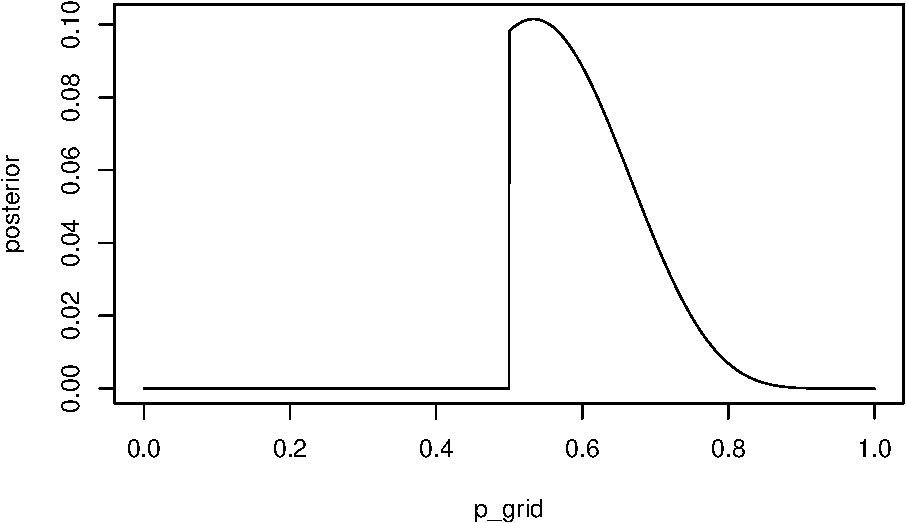
\includegraphics{_main_files/figure-latex/solve_3M5-1.pdf}

Сега добиваме \emph{posterior} дистрибуција која што за вредностите на параметарот под 0.5 практично кажува дека нема шанси да се случат.

\begin{Shaded}
\begin{Highlighting}[]
\NormalTok{samples }\OtherTok{\textless{}{-}} \FunctionTok{sample}\NormalTok{( p\_grid , }\AttributeTok{prob=}\NormalTok{posterior\_3m5 , }\AttributeTok{size=}\FloatTok{1e4}\NormalTok{ , }\AttributeTok{replace=}\ConstantTok{TRUE}\NormalTok{ )}

\FunctionTok{HPDI}\NormalTok{( samples , }\AttributeTok{prob=}\FloatTok{0.9}\NormalTok{ )}
\end{Highlighting}
\end{Shaded}

\begin{verbatim}
##      |0.9      0.9| 
## 0.5005005 0.7167167
\end{verbatim}

\emph{HPDI} интервалот исто така е многу потесен споредено со 3М2.

\emph{3M6. Suppose you want to estimate the Earth's proportion of water very precisely. Specifically, you want the 99\% percentile interval of the posterior distribution of p to be only 0.05 wide. This means the distance between the upper and lower bound of the interval should be 0.05. How many times will you have to toss the globe to do this?}

Ова решение го презедов од решенијата што ги пишува Richard McEarleth. Не ми беше јасно прашањето се додека не видов што прави кодот во решението.

Во овој проблем, всушност непознато е колку обзервации треба да направиме за да ја добиеме саканата прецизност. Решението е такво што \emph{ја бара} прецизност на серија обзервации (од 20 до 2000).

\begin{Shaded}
\begin{Highlighting}[]
\NormalTok{f }\OtherTok{\textless{}{-}} \ControlFlowTok{function}\NormalTok{(N) \{}
\NormalTok{  p\_true }\OtherTok{\textless{}{-}} \FloatTok{0.7}
\NormalTok{  W }\OtherTok{\textless{}{-}} \FunctionTok{rbinom}\NormalTok{(}\DecValTok{1}\NormalTok{, }\AttributeTok{size =}\NormalTok{ N, }\AttributeTok{prob =}\NormalTok{ p\_true)}
\NormalTok{  prob\_grid }\OtherTok{\textless{}{-}} \FunctionTok{seq}\NormalTok{(}\DecValTok{0}\NormalTok{, }\DecValTok{1}\NormalTok{, }\AttributeTok{length.out =} \DecValTok{1000}\NormalTok{)}
\NormalTok{  prior }\OtherTok{\textless{}{-}} \FunctionTok{rep}\NormalTok{(}\DecValTok{1}\NormalTok{, }\DecValTok{1000}\NormalTok{)}
\NormalTok{  prob\_data }\OtherTok{\textless{}{-}} \FunctionTok{dbinom}\NormalTok{(W, }\AttributeTok{size =}\NormalTok{ N, }\AttributeTok{prob =}\NormalTok{ prob\_grid)}
\NormalTok{  posterior }\OtherTok{\textless{}{-}}\NormalTok{ prob\_data }\SpecialCharTok{*}\NormalTok{ prior}
\NormalTok{  posterior }\OtherTok{\textless{}{-}}\NormalTok{ posterior }\SpecialCharTok{/} \FunctionTok{sum}\NormalTok{(posterior)}
\NormalTok{  samples }\OtherTok{\textless{}{-}} \FunctionTok{sample}\NormalTok{(p\_grid, }\AttributeTok{prob =}\NormalTok{ posterior, }\AttributeTok{size =} \FloatTok{1e4}\NormalTok{, }\AttributeTok{replace =} \ConstantTok{TRUE}\NormalTok{)}
\NormalTok{  PI99 }\OtherTok{\textless{}{-}} \FunctionTok{PI}\NormalTok{(samples, .}\DecValTok{99}\NormalTok{)}
  \FunctionTok{as.numeric}\NormalTok{(PI99[}\DecValTok{2}\NormalTok{] }\SpecialCharTok{{-}}\NormalTok{ PI99[}\DecValTok{1}\NormalTok{])}
\NormalTok{\}}
\NormalTok{Nlist }\OtherTok{\textless{}{-}} \FunctionTok{c}\NormalTok{(}\DecValTok{20}\NormalTok{, }\DecValTok{50}\NormalTok{, }\DecValTok{100}\NormalTok{, }\DecValTok{200}\NormalTok{, }\DecValTok{500}\NormalTok{, }\DecValTok{1000}\NormalTok{, }\DecValTok{2000}\NormalTok{)}
\NormalTok{Nlist }\OtherTok{\textless{}{-}} \FunctionTok{rep}\NormalTok{(Nlist, }\AttributeTok{each =} \DecValTok{100}\NormalTok{)}
\NormalTok{width }\OtherTok{\textless{}{-}} \FunctionTok{sapply}\NormalTok{(Nlist, f)}
\FunctionTok{plot}\NormalTok{(Nlist, width)}
\FunctionTok{abline}\NormalTok{(}\AttributeTok{h =} \FloatTok{0.05}\NormalTok{, }\AttributeTok{col =} \StringTok{"red"}\NormalTok{)}
\end{Highlighting}
\end{Shaded}

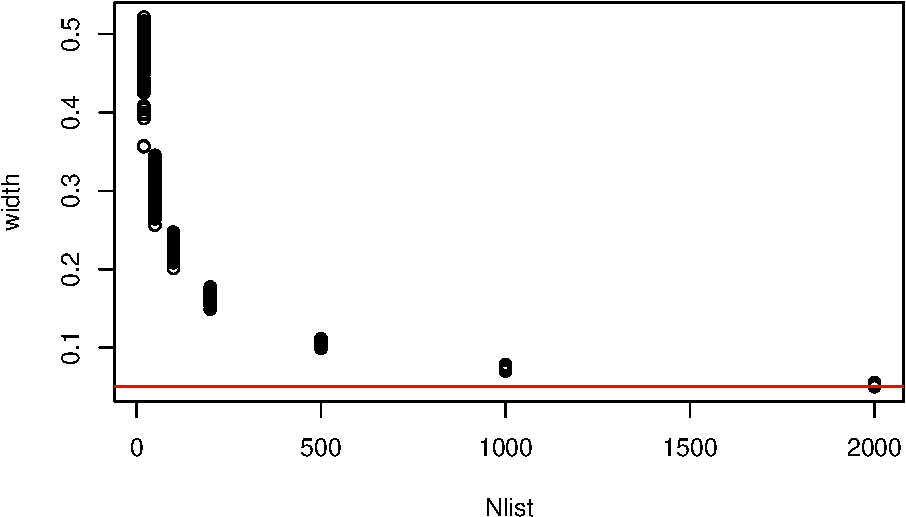
\includegraphics{_main_files/figure-latex/solve_3M6-1.pdf}

\emph{3H1. Using grid approximation, compute the posterior distribution for the probability of a birth being a boy. Assume a uniform prior probability.}

\begin{Shaded}
\begin{Highlighting}[]
\FunctionTok{data}\NormalTok{(homeworkch3)}

\NormalTok{all\_boys }\OtherTok{\textless{}{-}} \FunctionTok{sum}\NormalTok{(birth1) }\SpecialCharTok{+} \FunctionTok{sum}\NormalTok{(birth2)}
\end{Highlighting}
\end{Shaded}

\begin{Shaded}
\begin{Highlighting}[]
\NormalTok{p\_grid }\OtherTok{\textless{}{-}} \FunctionTok{seq}\NormalTok{( }\AttributeTok{from=}\DecValTok{0}\NormalTok{ , }\AttributeTok{to=}\DecValTok{1}\NormalTok{ , }\AttributeTok{length.out=}\DecValTok{1000}\NormalTok{ )}

\NormalTok{prior3h1 }\OtherTok{\textless{}{-}}\NormalTok{ prior }\OtherTok{\textless{}{-}} \FunctionTok{rep}\NormalTok{(}\DecValTok{1}\NormalTok{,}\FunctionTok{length}\NormalTok{(p\_grid))}

\NormalTok{likelihood }\OtherTok{\textless{}{-}} \FunctionTok{dbinom}\NormalTok{( all\_boys , }\AttributeTok{size=}\FunctionTok{length}\NormalTok{(birth1) }\SpecialCharTok{+} \FunctionTok{length}\NormalTok{(birth2) , }\AttributeTok{prob=}\NormalTok{p\_grid )}

\NormalTok{posterior }\OtherTok{\textless{}{-}}\NormalTok{ likelihood }\SpecialCharTok{*}\NormalTok{ prior3h1}

\NormalTok{posterior\_3h1 }\OtherTok{\textless{}{-}}\NormalTok{ posterior }\SpecialCharTok{/} \FunctionTok{sum}\NormalTok{(posterior)}

\FunctionTok{plot}\NormalTok{(p\_grid, posterior\_3h1 , }\AttributeTok{type=}\StringTok{"l"}\NormalTok{ )}
\FunctionTok{abline}\NormalTok{( }\AttributeTok{v=}\FloatTok{0.5}\NormalTok{ , }\AttributeTok{lty=}\DecValTok{2}\NormalTok{ )}
\end{Highlighting}
\end{Shaded}

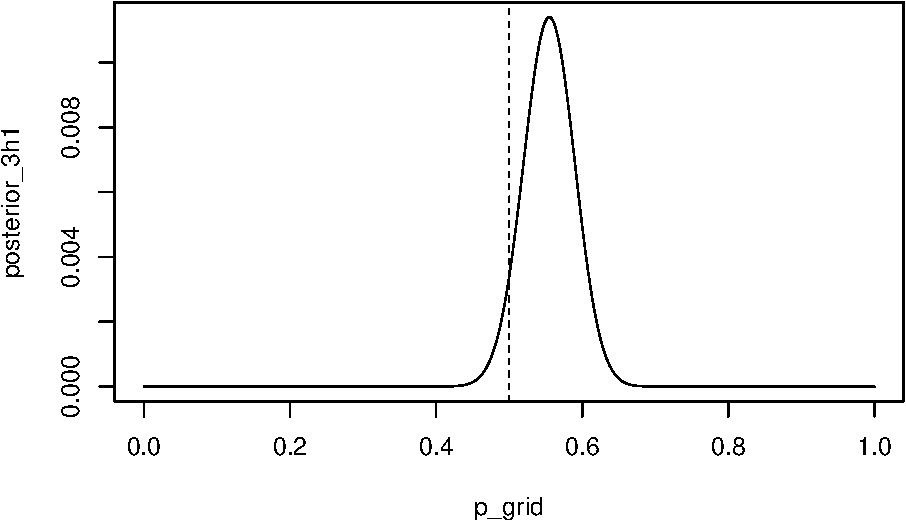
\includegraphics{_main_files/figure-latex/solve_3H1-1.pdf}

\emph{Which parameter value maximizes the posterior probability?}

\begin{Shaded}
\begin{Highlighting}[]
\NormalTok{p\_grid[ }\FunctionTok{which.max}\NormalTok{(posterior) ]}
\end{Highlighting}
\end{Shaded}

\begin{verbatim}
## [1] 0.5545546
\end{verbatim}

Можеби интересно да се види како ова би се напишало во \texttt{tidyverse} код:

\begin{Shaded}
\begin{Highlighting}[]
\NormalTok{data\_for\_3h1 }\OtherTok{\textless{}{-}}
  \FunctionTok{tibble}\NormalTok{(}\AttributeTok{p\_grid\_3h1 =} \FunctionTok{seq}\NormalTok{(}\AttributeTok{from =} \DecValTok{0}\NormalTok{, }\AttributeTok{to =} \DecValTok{1}\NormalTok{, }\AttributeTok{length.out =} \DecValTok{1000}\NormalTok{)) }\SpecialCharTok{\%\textgreater{}\%} 
  \FunctionTok{mutate}\NormalTok{(}\AttributeTok{prior\_3h1 =} \DecValTok{1}\NormalTok{) }\SpecialCharTok{\%\textgreater{}\%} 
  \FunctionTok{mutate}\NormalTok{(}\AttributeTok{data\_for\_3h1 =} \FunctionTok{dbinom}\NormalTok{( all\_boys , }\AttributeTok{size=}\FunctionTok{length}\NormalTok{(birth1) }\SpecialCharTok{+} \FunctionTok{length}\NormalTok{(birth2) , }\AttributeTok{prob=}\NormalTok{p\_grid\_3h1 )) }\SpecialCharTok{\%\textgreater{}\%} 
  \FunctionTok{mutate}\NormalTok{(}\AttributeTok{posterior\_3h1 =}\NormalTok{ data\_for\_3h1 }\SpecialCharTok{*}\NormalTok{ prior\_3h1) }\SpecialCharTok{\%\textgreater{}\%} 
  \FunctionTok{mutate}\NormalTok{(}\AttributeTok{posterior\_3h1\_st =}\NormalTok{ posterior\_3h1 }\SpecialCharTok{/} \FunctionTok{sum}\NormalTok{(posterior\_3h1))}
\end{Highlighting}
\end{Shaded}

\begin{Shaded}
\begin{Highlighting}[]
\FunctionTok{ggplot}\NormalTok{(data\_for\_3h1) }\SpecialCharTok{+} 
  \FunctionTok{aes}\NormalTok{(}\AttributeTok{x =}\NormalTok{ p\_grid\_3h1, }\AttributeTok{y =}\NormalTok{ posterior\_3h1\_st) }\SpecialCharTok{+}
  \FunctionTok{geom\_line}\NormalTok{() }\SpecialCharTok{+}
  \FunctionTok{theme\_minimal}\NormalTok{()}
\end{Highlighting}
\end{Shaded}

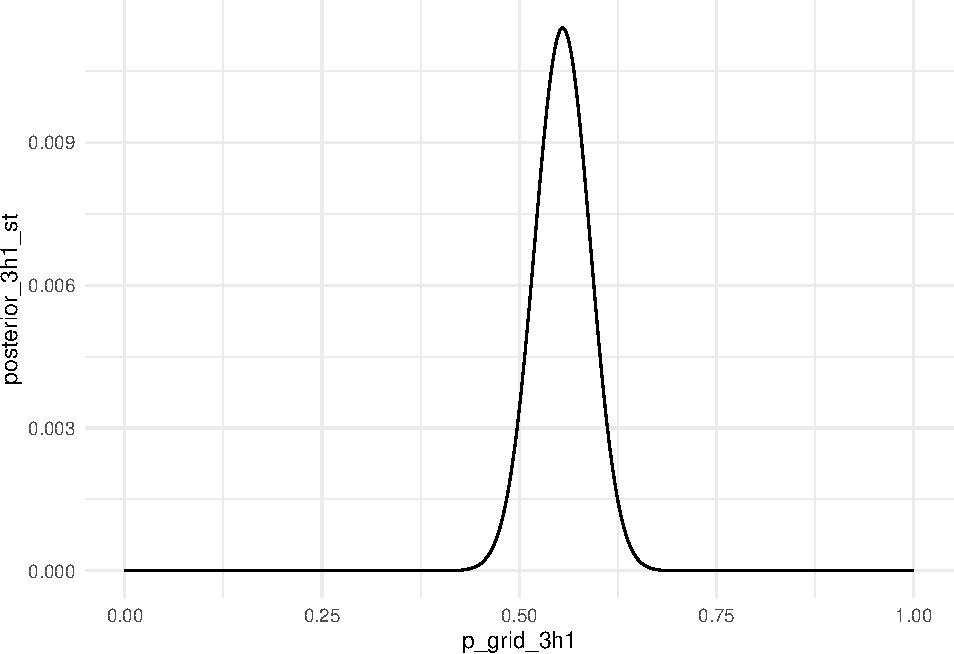
\includegraphics{_main_files/figure-latex/solve_3H1_3-1.pdf}

\emph{3H2. Using the sample function, draw 10,000 random parameter values from the posterior distribution you calculated above. Use these samples to estimate the 50\%, 89\%, and 97\% highest posterior density intervals.}

\begin{Shaded}
\begin{Highlighting}[]
\NormalTok{samples }\OtherTok{\textless{}{-}} \FunctionTok{sample}\NormalTok{( data\_for\_3h1}\SpecialCharTok{$}\NormalTok{p\_grid\_3h1 , }\AttributeTok{prob=}\NormalTok{data\_for\_3h1}\SpecialCharTok{$}\NormalTok{posterior\_3h1\_st , }\AttributeTok{size=}\FloatTok{1e4}\NormalTok{ , }\AttributeTok{replace=}\ConstantTok{TRUE}\NormalTok{ )}

\FunctionTok{plot}\NormalTok{(samples)}
\end{Highlighting}
\end{Shaded}

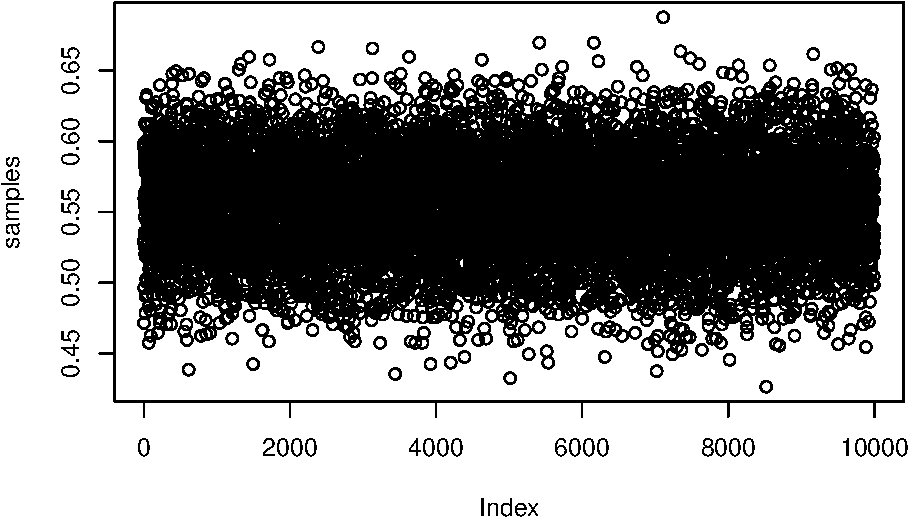
\includegraphics{_main_files/figure-latex/solve_3H2-1.pdf}

\begin{Shaded}
\begin{Highlighting}[]
\NormalTok{tidybayes}\SpecialCharTok{::}\FunctionTok{hdi}\NormalTok{(samples, }\AttributeTok{.width =}\NormalTok{ .}\DecValTok{50}\NormalTok{)}
\end{Highlighting}
\end{Shaded}

\begin{verbatim}
##           [,1]      [,2]
## [1,] 0.5255255 0.5725726
\end{verbatim}

\begin{Shaded}
\begin{Highlighting}[]
\NormalTok{tidybayes}\SpecialCharTok{::}\FunctionTok{hdi}\NormalTok{(samples, }\AttributeTok{.width =}\NormalTok{ .}\DecValTok{89}\NormalTok{)}
\end{Highlighting}
\end{Shaded}

\begin{verbatim}
##           [,1]      [,2]
## [1,] 0.5005005 0.6126126
\end{verbatim}

\begin{Shaded}
\begin{Highlighting}[]
\NormalTok{tidybayes}\SpecialCharTok{::}\FunctionTok{hdi}\NormalTok{(samples, }\AttributeTok{.width =}\NormalTok{ .}\DecValTok{97}\NormalTok{)}
\end{Highlighting}
\end{Shaded}

\begin{verbatim}
##           [,1]      [,2]
## [1,] 0.4774775 0.6276276
\end{verbatim}

\emph{3H3. Use rbinom to simulate 10,000 replicates of 200 births. You should end up with 10,000 numbers, each one a count of boys out of 200 births. Compare the distribution of predicted numbers of boys to the actual count in the data (111 boys out of 200 births). There are many good ways to visualize the simulations, but the dens command (part of the rethinking package) is probably the easiest way in this case. Does it look like the model fits the data well? That is, does the distribution of predictions include the actual observation as a central, likely outcome?}

\begin{Shaded}
\begin{Highlighting}[]
\NormalTok{simulate }\OtherTok{\textless{}{-}} \FunctionTok{tibble}\NormalTok{(}\AttributeTok{births =} \FunctionTok{rbinom}\NormalTok{( }\DecValTok{10000}\NormalTok{ , }\AttributeTok{size=}\DecValTok{200}\NormalTok{ , }\AttributeTok{prob=}\NormalTok{samples ))}

\FunctionTok{ggplot}\NormalTok{(simulate) }\SpecialCharTok{+} 
  \FunctionTok{aes}\NormalTok{(}\AttributeTok{x =}\NormalTok{ births) }\SpecialCharTok{+}
  \FunctionTok{geom\_density}\NormalTok{() }\SpecialCharTok{+}
  \FunctionTok{theme\_minimal}\NormalTok{() }\SpecialCharTok{+}
  \FunctionTok{geom\_vline}\NormalTok{(}\AttributeTok{xintercept =} \FunctionTok{sum}\NormalTok{(birth1 }\SpecialCharTok{+}\NormalTok{ birth2), }\AttributeTok{color =} \StringTok{"red"}\NormalTok{) }\SpecialCharTok{+}
  \FunctionTok{geom\_vline}\NormalTok{(}\AttributeTok{xintercept =} \FunctionTok{mean}\NormalTok{(simulate}\SpecialCharTok{$}\NormalTok{births, }\AttributeTok{na.rm =} \ConstantTok{TRUE}\NormalTok{), }\AttributeTok{color =} \StringTok{"blue"}\NormalTok{) }\SpecialCharTok{+}
  \FunctionTok{labs}\NormalTok{(}\AttributeTok{caption =} \StringTok{"Blue line is mean of simulated data, red line is number of boys from data."}\NormalTok{)}
\end{Highlighting}
\end{Shaded}

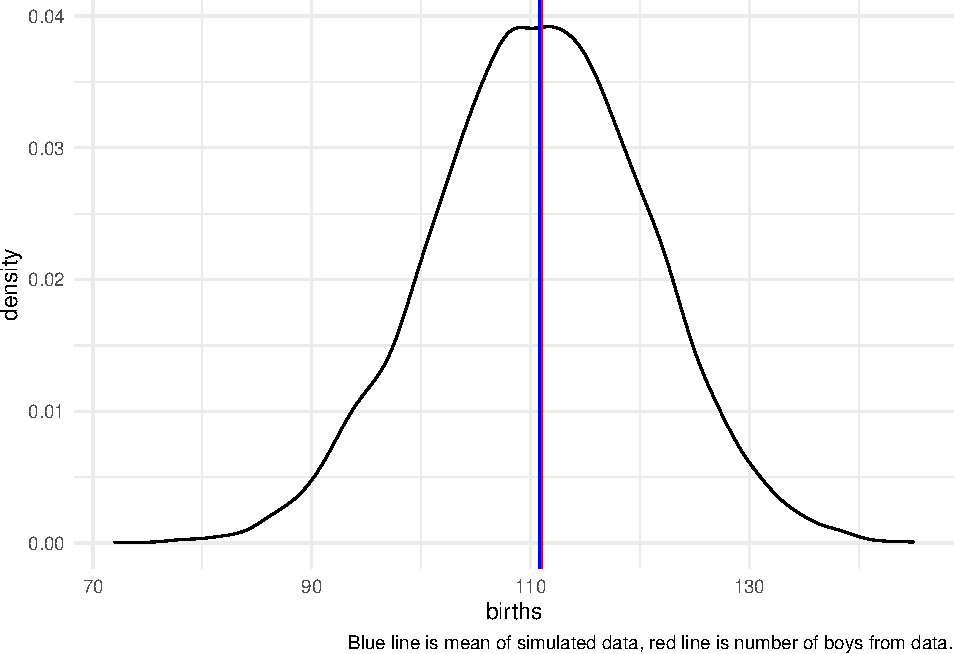
\includegraphics{_main_files/figure-latex/solve_3H3-1.pdf}

\emph{3H4. Now compare 10,000 counts of boys from 100 simulated first-borns only to the number of boys in the first births, birth1. How does the model look in this light?}

\begin{Shaded}
\begin{Highlighting}[]
\NormalTok{simulate }\OtherTok{\textless{}{-}} \FunctionTok{tibble}\NormalTok{(}\AttributeTok{births =} \FunctionTok{rbinom}\NormalTok{( }\DecValTok{10000}\NormalTok{ , }\AttributeTok{size=}\DecValTok{100}\NormalTok{ , }\AttributeTok{prob=}\NormalTok{samples ))}

\FunctionTok{ggplot}\NormalTok{(simulate) }\SpecialCharTok{+} 
  \FunctionTok{aes}\NormalTok{(}\AttributeTok{x =}\NormalTok{ births) }\SpecialCharTok{+}
  \FunctionTok{theme\_minimal}\NormalTok{() }\SpecialCharTok{+}
  \FunctionTok{geom\_density}\NormalTok{() }\SpecialCharTok{+}
  \FunctionTok{geom\_vline}\NormalTok{(}\AttributeTok{xintercept =} \FunctionTok{sum}\NormalTok{(birth1), }\AttributeTok{color =} \StringTok{"red"}\NormalTok{) }\SpecialCharTok{+}
  \FunctionTok{geom\_vline}\NormalTok{(}\AttributeTok{xintercept =} \FunctionTok{mean}\NormalTok{(simulate}\SpecialCharTok{$}\NormalTok{births, }\AttributeTok{na.rm =} \ConstantTok{TRUE}\NormalTok{), }\AttributeTok{color =} \StringTok{"blue"}\NormalTok{) }\SpecialCharTok{+}
  \FunctionTok{labs}\NormalTok{(}\AttributeTok{caption =} \StringTok{"Blue line is mean of simulated data, red line is number of first{-}born boys from data."}\NormalTok{)}
\end{Highlighting}
\end{Shaded}

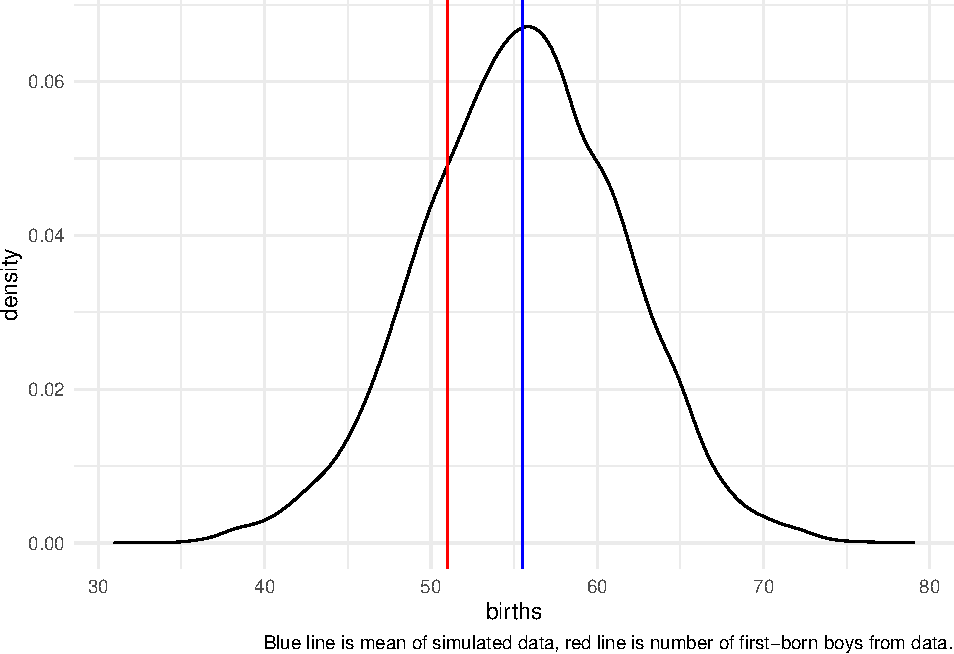
\includegraphics{_main_files/figure-latex/solve_3H4-1.pdf}

\emph{3H5. The model assumes that sex of first and second births are independent. To check this assumption, focus now on second births that followed female first borns. Compare 10,000 simulated counts of boys to only those second births that followed girls. To do this correctly, you need to count the number of first borns who were girls and simulate that many births, 10,000 times. Compare the counts of boys in your simulations to the actual observed count of boys following girls. How does the model look in this light? Any guesses what is going on in these data?}

\begin{Shaded}
\begin{Highlighting}[]
\NormalTok{first\_born\_girls }\OtherTok{\textless{}{-}} \FunctionTok{sum}\NormalTok{(birth1}\SpecialCharTok{==}\DecValTok{0}\NormalTok{)}

\NormalTok{simulate }\OtherTok{\textless{}{-}} \FunctionTok{tibble}\NormalTok{(}\AttributeTok{births =} \FunctionTok{rbinom}\NormalTok{(}\DecValTok{10000}\NormalTok{, }\AttributeTok{size=}\NormalTok{first\_born\_girls, }\AttributeTok{prob=}\NormalTok{samples))}

\FunctionTok{ggplot}\NormalTok{(simulate) }\SpecialCharTok{+} 
  \FunctionTok{aes}\NormalTok{(}\AttributeTok{x =}\NormalTok{ births) }\SpecialCharTok{+}
  \FunctionTok{geom\_density}\NormalTok{() }\SpecialCharTok{+}
  \FunctionTok{theme\_minimal}\NormalTok{() }\SpecialCharTok{+}
  \FunctionTok{geom\_vline}\NormalTok{(}\AttributeTok{xintercept =} \FunctionTok{sum}\NormalTok{(birth1 }\SpecialCharTok{+}\NormalTok{ birth2), }\AttributeTok{color =} \StringTok{"red"}\NormalTok{) }\SpecialCharTok{+}
  \FunctionTok{geom\_vline}\NormalTok{(}\AttributeTok{xintercept =} \FunctionTok{mean}\NormalTok{(simulate}\SpecialCharTok{$}\NormalTok{births, }\AttributeTok{na.rm =} \ConstantTok{TRUE}\NormalTok{), }\AttributeTok{color =} \StringTok{"blue"}\NormalTok{) }\SpecialCharTok{+}
  \FunctionTok{labs}\NormalTok{(}\AttributeTok{caption =} \StringTok{"Blue line is mean of simulated data, red line is number of first{-}born girls from data."}\NormalTok{)}
\end{Highlighting}
\end{Shaded}

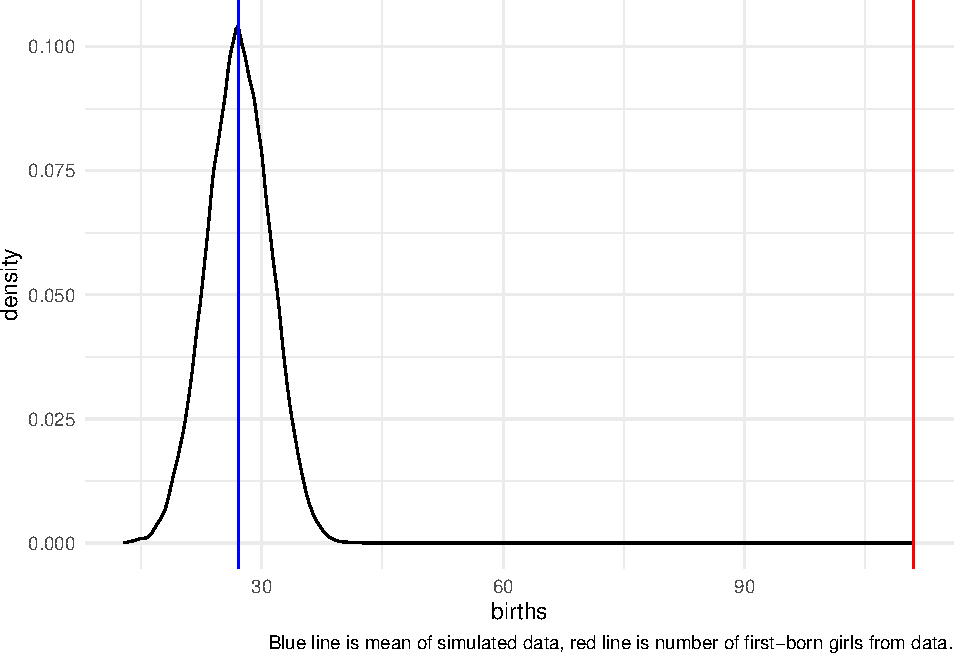
\includegraphics{_main_files/figure-latex/solve_3H5-1.pdf}

  \bibliography{book.bib,packages.bib}

\end{document}
